\documentclass{llncs}
\usepackage{amsmath,amssymb,amsfonts}
\usepackage{booktabs}
\usepackage{multirow}
\usepackage{graphicx}
\usepackage{textcomp}
\usepackage{xcolor}
\usepackage[printonlyused]{acronym}
\usepackage{orcidlink}
\usepackage{placeins}
\acrodef{HRC}{Human--Robot Collaboration}
\acrodef{EEG}{Electroencephalography}
\acrodef{EMG}{Electromyography}
\acrodef{EDA}{Electrodermal Activity}
\acrodef{ECG}{Electrocardiography}
\acrodef{AI}{Artificial Intelligence}
\acrodef{XGBoost}{eXtreme Gradient Boosting}
\acrodef{MLP}{Multilayer Perceptron}
\acrodef{LOSO}{Leave-One-Subject-Out}
\acrodef{OOF}{out-of-fold}
\acrodef{SVM}{Support Vector Machine}
\acrodef{ECE}{Expected Calibration Error}
\acrodef{F1}{F1-score}

\graphicspath{{figures/}}

\begin{document}

\title{Recognizing Operator Task States from Multimodal Physiological Signals in Industrial Human--Robot Collaboration:\ a Subject-Disjoint Evaluation}

\author{Ameur Gargouri\inst{1}\orcidlink{0009-0001-8293-037X} \and Mohamed Karray\inst{2}\orcidlink{0000-0001-7293-8696} \and Mohamed Ksantini\inst{3}\orcidlink{0000-0002-9928-8643}}

\institute{ESME Research Lab \\
ATISP Laboratory, ENET'Com\\
University of Sfax\\
Ivry-sur-Seine, France / Sfax, Tunisia\\
\email{ameur.gargouri.doc@enetcom.usf.tn}
\and
ESME Research Lab\\
Ivry-sur-Seine, France\\
\email{mohamed.karray@esme.fr}
\and
ATISP Laboratory, ENET'Com\\
University of Sfax\\
Sfax, Tunisia\\
\email{mohamed.ksantini@ipeis.usf.tn}}
\maketitle

\begin{abstract}
Collaborative and assistive robots that share a workspace with a human operator must react not only to the geometry of the task but to the state of the person performing it: whether the operator is cognitively loaded, stressed, or engaged in a demanding physical manipulation changes what kind of assistance is useful and when it should be offered. Physiological signals, such as brain activity through \ac{EEG} and autonomic arousal through \ac{ECG}, \ac{EDA}, \ac{EMG}, and respiration, provide a continuous, non-intrusive window onto these states. Yet a core challenge prevents such signals from driving adaptation in practice: most reported evaluations do not transfer to new operators. Windows of the same operator are commonly split at random between training and test, recording metadata leaks into the feature matrix, and the between-operator variability that dominates real deployments is left unquantified. We propose, in this paper, a leakage-free, strictly subject-disjoint evaluation of task-state recognition on the public MultiPhysio-\ac{HRC} dataset. Results show that gradient boosting achieves the best across-operator macro-F1 of $0.466\pm0.149$, statistically tied with \ac{XGBoost}, while within-subject classifiers on the identical features reach $0.91$, an operator-induced gap of roughly $0.45$ points that dwarfs every other factor in the error budget. Fusing \ac{EEG} and peripheral features consistently and significantly outperforms the best single modality, and all detectors classify a window in at most $\sim$90\,$\mu$s, confirming real-time feasibility.
\keywords{physiological signals \and task-type recognition \and multimodal fusion \and human-robot collaboration \and subject-disjoint evaluation \and reproducibility}
\end{abstract}

\section{Introduction}
\label{sec:intro}

In shared and assistive \ac{HRC}, a robot and an operator work on the same physical
task and must coordinate in real time. Coordinating well requires the robot to
interpret not only the geometric state of the shared workspace but also the state of
the person working in it: whether an operator is under high mental load, stressed, or
performing a demanding physical manipulation changes what kind of assistance is useful
and how it should be timed \cite{selvaggio2021autonomy}. Physiological signals offer a
continuous and non-disruptive window onto these states, such as brain activity through
\ac{EEG} and autonomic arousal through \ac{ECG}, \ac{EDA}, \ac{EMG}, and
respiration, and are increasingly used to drive adaptive behaviour in collaborative
robotics \cite{bussolan2024stressdetector,borghi2025operatorstress}.

The task we address is \emph{task-state recognition}: given a window of physiological
signals, decide which kind of activity the operator is engaged in. We deliberately use
coarse, task-condition classes, namely a cognitive-load battery, a stressor, an
industrial physical task, rest, and a residual class, rather than fine-grained
continuous
states, because coarse classes are the actionable unit for an assistive policy and
because they are exactly what the recording protocol can certify without invasive
labelling. Yet even this deliberately simple formulation is hard in practice, for two
reasons that shape everything that follows. \emph{Operator dependence}: physiological
baselines and response magnitudes differ sharply between individuals, so a model
trained on one set of operators can appear excellent on a random held-out subset of
\emph{the same} operators' windows while failing on a genuinely new operator. Any
evaluation that does not separate operators risks reporting a ceiling rather than a
generalization result. \emph{Class imbalance}: in the data we use, one class,
industrial task, accounts for 63\% of windows while two minority classes together
account for 5\%, which makes aggregate accuracy uninformative without class-level
controls.

Recognition of physiological operator state has been pursued along three main lines,
each of which leaves a distinct gap open. Subject-state methods train on
questionnaire-labelled stress and cognitive-load reports and consistently observe that
recognition across operators is hard, but they inherit the subjectivity and the
coverage of self-reports
\cite{bussolan2025multiphysiohrc,bussolan2024stressdetector,borghi2025operatorstress,aygun2022assistive}.
Fusion methods argue that central and peripheral modalities carry complementary
information, yet the argument is mostly taxonomic and rarely tested under a controlled
design on data where channels are heavily redundant \cite{baltrusaitis2019multimodal}.
Evaluation-centred reviews have shown that the design of the data split is the single
largest driver of reported performance, but they stop at cataloguing the heterogeneity
rather than supplying a clean protocol
\cite{jin2025cognitivestate,iarlori2024cognitiveworkload}.

In spite of these advances, some issues still exist. Firstly, evaluations of
physiological windows are frequently not subject-disjoint: repeated, auto-correlated
windows from the same operator and the same condition are split randomly between
training and test, and metadata such as recording identifiers leak into the feature
matrix. The resulting numbers are flattering and irreproducible. Secondly, the
between-operator variability that practitioners actually face is rarely quantified: a
reader of most papers cannot tell what fraction of the reported accuracy reflects
recognition of the \emph{task} and what fraction reflects recognition of the
\emph{person}, because no within-subject upper bound is reported alongside the
across-operator result. Thirdly, fusion of central and peripheral physiology is
generally asserted to help, but the claim is rarely tested with a modality ablation
under the identical cleaning and protocol.

This paper addresses these gaps by proposing a leakage-free, strictly subject-disjoint
benchmark of task-state recognition on the public MultiPhysio-\ac{HRC} dataset. We
first audit the exported feature table and remove 112 columns that are recording
metadata or byte-identical duplicated \ac{EEG} exports, leaving 128 physiological
features, and we label each window deterministically from its protocol condition into
one of five task-condition classes. We then evaluate eleven off-the-shelf detectors
and one neural fusion architecture under a \ac{LOSO} protocol over all 52 operators,
refitting every preprocessing step inside each training fold, and we keep a
within-subject run on the identical features only as an explicit upper bound. The
headline finding is honest and, we believe, useful: the best detector reaches a
per-fold macro-F1 of $0.466\pm0.149$ across new operators, whereas within-subject
classifiers on the same features reach $0.91$, a generalization gap of roughly $0.45$
points that dwarfs the differences between models. A modality ablation under the same
protocol shows that fusing \ac{EEG} with peripheral signals adds a small but
significant gain over the best single modality, and that explicit two-tower fusion
does not beat plain concatenation. Finally, all detectors classify a window in at most
a few tens of microseconds, so real-time assistance is not constrained by inference
cost. The contributions are:

\begin{enumerate}
\item a \textbf{leakage-free feature-cleaning protocol} for a public
physiological-\ac{HRC} dataset, together with a machine-readable manifest
recording, for every feature, its modality group and its keep/drop decision with the
reason, and a deterministic five-class task-condition labelling rule.
\item a \textbf{strictly subject-disjoint \ac{LOSO} benchmark} of eleven classical and
neural detectors over all 52 operators, with preprocessing refit inside each fold,
per-fold score files, paired significance tests, and calibration reporting, alongside
a within-subject run kept as an explicit upper bound.
\item a \textbf{modality-contribution analysis} under this protocol that answers,
under a controlled design, whether fusion of central and peripheral physiology
actually helps.
\item a quantitative statement of the \textbf{generalization gap} between within-subject
and across-operator performance, together with real-time latency figures, a deployment
and privacy discussion, and a released reproducibility package.
\end{enumerate}

The rest of this paper is structured in the following manner. Section~\ref{sec:related}
reviews related work. Section~\ref{sec:dataset} describes the dataset, the feature
audit, and the label schema. Section~\ref{sec:method} details the models and the
\ac{LOSO} evaluation protocol. Section~\ref{sec:results} reports results and
Section~\ref{sec:discussion} discusses them and the threats to validity.
Section~\ref{sec:conclusion} concludes with implications and future directions.

\section{Related Work}
\label{sec:related}

Physiological operator-state recognition for \ac{HRC} has seen significant advances
through datasets, fusion models, and evaluation studies. This section outlines recent
contributions in each of these areas while highlighting the unique drawbacks that
motivate the present work.

Bussolan et al.~\cite{bussolan2025multiphysiohrc} introduced the MultiPhysio-\ac{HRC}
dataset used in this paper and reported subject-disjoint recognition of
\emph{self-reported} stress and cognitive-load levels on an industrial assembly task,
reaching macro-F1 ranges of roughly 0.34--0.39 for stress and 0.33--0.49 for cognitive
load across conditions \cite{bussolan2024stressdetector}. These modest numbers,
obtained with questionnaire ground truth under a subject-disjoint protocol, are an
important reference point: they indicate that across-operator physiological
recognition is genuinely hard and that honest protocols produce honest results.
However, their targets come from STAI-Y1/NASA-TLX self-reports that are not part of
the public feature export, the protocol covers a narrower assembly setting, and the
source study neither audits its feature export for leakage nor tests whether fusing
modalities helps under a controlled design.

Borghi et al.~\cite{borghi2025operatorstress} assessed operator stress in collaborative
robotics with a multimodal approach and likewise insist on careful subject-independent
evaluation, reporting large variance across individuals. Aygun et al.~\cite{aygun2022assistive}
estimated cognitive workload for assistive robots from physiological signals and again
observed pronounced between-subject variability. These works establish that the
operator effect is the central difficulty, but they evaluate single-target states on
single-architecture pipelines, so the relative contribution of features, fusion, and
evaluation design remains entangled.

On the fusion side, Baltrusaitis et al.~\cite{baltrusaitis2019multimodal} provide the
standard taxonomy of multimodal machine learning, arguing that heterogeneous streams
carry complementary information and that naive fusion can hurt when modalities are
redundant or noisy. The taxonomy is largely descriptive: controlled \emph{empirical}
tests on physiological-\ac{HRC} data, where redundancy across channels is high and the
fusion benefit is not guaranteed, are scarce. Our modality-contribution analysis is a
step toward filling that gap.

On the evaluation side, Iarlori et al.~\cite{iarlori2024cognitiveworkload} survey
cognitive-workload estimation from wearables in human--machine interaction and
catalogue the evaluation heterogeneity that makes studies hard to compare.
Jin et al.~\cite{jin2025cognitivestate} provide a recent systematic review of
physiological cognitive-state recognition and show that the design of the data split
is the single largest driver of reported performance differences. These reviews
identify the disease but do not supply the cure: neither proposes a concrete,
reproducible subject-disjoint protocol with an explicit within-subject upper bound.

Finally, Selvaggio et al.~\cite{selvaggio2021autonomy} survey autonomy levels in
physical human--robot interaction and identify reliability, transparency, and
adaptation as the constraints any state estimator must serve. Task-state recognition
is a building block of such autonomy, and our latency and failure-mode analysis speaks
to the deployment requirements they enumerate.

In summary, prior work establishes that fusion of physiological modalities is
promising in principle \cite{baltrusaitis2019multimodal}, that operator-state
recognition in \ac{HRC} is hard and subject-dependent
\cite{bussolan2025multiphysiohrc,bussolan2024stressdetector,borghi2025operatorstress,aygun2022assistive},
and that evaluation design determines reported performance
\cite{jin2025cognitivestate,iarlori2024cognitiveworkload}. What is missing is a
compact, reproducible, subject-disjoint benchmark of task-condition recognition on a
public \ac{HRC} dataset that simultaneously audits the features, tests whether fusion
helps, and quantifies the within-subject versus across-operator gap. The present work
directly addresses this gap.

\section{Dataset and Task Formulation}
\label{sec:dataset}

\subsection{MultiPhysio-\ac{HRC}}

We use the public MultiPhysio-\ac{HRC} dataset of multimodal physiological recordings
collected during controlled and realistic industrial human--robot collaboration
\cite{bussolan2025multiphysiohrc}. It comprises 52 healthy operators who each
performed a battery of 21 protocol conditions while wearing a multi-sensor setup: an
\ac{EEG} headset plus peripheral sensors for \ac{ECG}, \ac{EDA}, \ac{EMG}, and
respiration. From the continuous recordings the dataset publishes fixed-duration
signal windows together with statistical descriptors. The export we obtained contains
5{,}640 windows, each originally carrying 257 columns.

\subsection{Auditing the feature export}

Before any modelling, we audited the exported feature table for the two most common
leakage sources in this kind of data.

First, \emph{recording-metadata leakage}. Sixteen columns aggregate the recording
identifier, \texttt{ID\_\_*}, and the trial counter, \texttt{Repetition\_\_*}. These
identify the recording session and its order, not the operator's physiology: they are
removed, because they would otherwise let a model short-circuit on trial metadata.
Second, \emph{duplicated \ac{EEG} features}. The export contains each \ac{EEG}
descriptor twice, once under a clean name and once under a
\texttt{eeg\_features\_5s\_\_...} prefix, byte-identical. The 96 duplicated columns are
removed so that \ac{EEG} is weighted exactly once.

The audit is summarized in Table~\ref{tab:audit}. After cleaning, the 128 remaining
physiological features are statistical descriptors, namely mean, standard deviation,
median, and energy, of windowed signals. A machine-readable manifest recording the decision
and the reason for every column is released with the reproducibility package.

\begin{table}[t]
\centering
\small
\caption{Feature-export audit. The 257 exported columns reduce to 128 physiological
features after removing 16 recording-metadata columns and 96 byte-identical duplicated
\ac{EEG} descriptors. The label columns are retained as keys. No model input is taken
from them.}
\label{tab:audit}
\begin{tabular}{lrr}
\toprule
Column group & Count & Disposition \\
\midrule
Physiological features, \ac{EEG} & 96 & kept \\
Physiological features, \ac{ECG} & 8 & kept \\
Physiological features, \ac{EDA} & 8 & kept \\
Physiological features, \ac{EMG} & 8 & kept \\
Physiological features, respiration & 8 & kept \\
\hline
\ac{EEG} duplicated descriptors & 96 & dropped, exact copies \\
Recording metadata, \texttt{ID\_\_*} and \texttt{Repetition\_\_*}, & 16 & dropped, leakage \\
\bottomrule
\end{tabular}
\end{table}

\subsection{Task-condition labels}

MultiPhysio-\ac{HRC} annotates each recording with the \emph{protocol condition} that
was performed and with self-report questionnaires. The questionnaires are not part of
the public feature export we obtained, so we do not claim to recognize self-reported
affective state. Instead, we define the recognition target as the \emph{task
condition}, which is certified by the experimental protocol itself: each window
receives exactly one of five labels, assigned deterministically from the recording's
\texttt{task\_name} by the rule in Table~\ref{tab:schema}, with the rule released
verbatim in the reproducibility package. Because the labels are a deterministic
function of the protocol, they are exact and reproducible: no crowdsourcing, no
subjective rating, no ambiguity about which condition a window came from.

The five classes are chosen so that every protocol condition maps to a class with a
coherent physiological hypothesis.

\begin{itemize}
\item \textbf{cognitive load}: 975 windows, a sustained-attention and memory battery,
namely Stroop easy/hard, N-back, Tower of Hanoi, and arithmetic/puzzle. These
conditions tax working memory and executive control.
\item \textbf{high stress}: 224 windows, a virtual-reality height-plank walking task,
a validated stressor inducing threat-related autonomic arousal.
\item \textbf{industrial task}: 3{,}571 windows, ten physical assembly and
order-picking conditions, five performed manually and five with a collaborative robot.
These mix physical and cognitive demands in realistic \ac{HRC} settings.
\item \textbf{low load}: 799 windows, rest and guided-meditation segments between
conditions, providing a low-demand baseline.
\item \textbf{other}: 71 windows, a single open-ended virtual-reality job-simulation
session that belongs to none of the controlled batteries. It is kept as its own class
rather than forced into another, and its small size is reported explicitly.
\end{itemize}

\begin{table}[t]
\centering
\small
\caption{Deterministic mapping from the 21 protocol conditions to the five
task-condition classes, with window counts. Every row of the cleaned data is labelled
by this rule. No crowdsourcing or manual labelling is involved.}
\label{tab:schema}
\begin{tabular}{@{}llr@{}}
\toprule
Class & Protocol conditions, \texttt{task\_name} & Windows \\
\midrule
\multirow{5}{*}{cognitive load} & \texttt{stroopeasy\_0} & 138 \\
 & \texttt{stroophard\_0} & 98 \\
 & \texttt{n-back\_0} & 204 \\
 & \texttt{hanoi\_0} & 337 \\
 & \texttt{mat\_0} & 198 \\
\multirow{1}{*}{high stress} & \texttt{vr-plank\_0} & 224 \\
\multirow{10}{*}{industrial task} & \texttt{manual-task-1}\dots\texttt{-5} & 1{,}587 \\
 & \texttt{cobot-task-1}\dots\texttt{-5} & 1{,}984 \\
\multirow{5}{*}{low load} & \texttt{rest-1},\,\texttt{rest-2},\,\texttt{rest\_0} & 654 \\
 & \texttt{meditation\_0} & 145 \\
\multirow{1}{*}{other} & \texttt{vr-job-sim\_0} & 71 \\
\midrule
 & Total & 5{,}640 \\
\bottomrule
\end{tabular}
\end{table}

The task is therefore \emph{well-posed but not trivial}: the five classes correspond
to different conditions, yet physiological differences across individuals are large
enough that a classifier must separate \emph{classes} from \emph{persons}. This is
precisely the separation that a subject-disjoint protocol enforces, described
in Section~\ref{sec:protocol}.

\section{Methodology}
\label{sec:method}

\subsection{Pipeline overview}

The processing and evaluation pipeline is shown in Figure~\ref{fig:pipeline}. A single
preprocessing path produces the fused tabular representation used by every detector.
Modality feature groups are kept separate alongside it so that the modality-contribution
analysis of Section~\ref{sec:results} reuses the identical path. All detectors share one
evaluation protocol, so any difference in outcome is attributable to the detector
itself rather than to the data preparation.

\begin{figure}[t]
\centering

\includegraphics[width=\textwidth]{task_pipeline.png}
\caption{Processing and evaluation pipeline. One clean preprocessing path feeds a
fused 128-dimensional tabular representation. The same path exposes modality feature
groups for the fusion ablation. All detectors are evaluated under the identical
subject-disjoint \ac{LOSO} protocol with preprocessing refit inside each fold.}
\label{fig:pipeline}
\end{figure}

\subsection{Problem formulation}

Let $\{x_i, y_i, s_i\}_{i=1}^{N}$ denote the cleaned windows, where
$x_i \in \mathbb{R}^{128}$ is the fused feature vector, $y_i \in
\mathcal{Y} = \{1,\dots,5\}$ is the task-condition label, with cognitive load $=1$,
high stress $=2$, industrial task $=3$, low load $=4$, and other $=5$, and
$s_i \in \{1,\dots,52\}$ is the operator who produced the window.
Two statistical facts about this data drive the design of the objective. Windows of
the same operator are not independent, and repeated windows of the same condition are
strongly autocorrelated. The class counts of Table~\ref{tab:schema} are heavily
imbalanced, with one majority class covering 63\% of the windows.

For a model $f_\theta$ producing class posteriors $p_\theta(y=c \mid x_i)$, we train
with the class-weighted cross-entropy objective
\begin{equation}
\mathcal{L}(\theta)\;=\;-\frac{1}{|\mathcal{B}|}\sum_{i\in\mathcal{B}}
\sum_{c=1}^{5} w_c\,\mathbf{1}[y_i=c]\;\log p_\theta(y=c\mid x_i),
\label{eq:loss}
\end{equation}
where $\mathcal{B}$ is a training batch, the full set for batch models, and
$w_c \propto N / (5\,N_c)$ is the inverse-frequency weight of class $c$ with
$N_c=\sum_i \mathbf{1}[y_i=c]$. The weights counteract the imbalance of
Table~\ref{tab:schema} so that the loss is not dominated by the majority
\emph{industrial task} class. Without them, a trivial constant classifier already
attains 63\% accuracy. The decision rule at test time is the maximum-posterior rule
\begin{equation}
\hat{y}_i \;=\; \arg\max_{c\in\mathcal{Y}}\; p_\theta(y=c \mid x_i),
\label{eq:argmax}
\end{equation}
which, together with the class weighting in Eq.~\eqref{eq:loss}, targets
class-balanced behaviour rather than raw accuracy.

\subsection{Preprocessing and feature representation}

Preprocessing is deliberately minimal and identical across models so that performance
differences are attributable to the detectors and to the protocol, not to bespoke
feature engineering:
\begin{enumerate}
\item columns audited as in Section~\ref{sec:dataset}, the 128 kept features forming
$x_i$.
\item missing values are imputed with the training-fold median, and the audit found
328 missing entries out of $5{,}640\times128$.
\item features are standardized to zero mean and unit variance using training-fold
statistics only, and
\item a fused representation is used by all tabular detectors, while the
modality-feature groups, \ac{EEG} and peripheral, are exposed to the ablation and to
the two-tower architecture.
\end{enumerate}
Crucially, imputation and standardization are \emph{refit inside every training fold},
as described in Section~\ref{sec:protocol}. Test operators never contribute to the
statistics that transform their own windows, which removes a subtle and common form of
leakage.

\subsection{Detectors}

To justify our choice of detectors: the aim is to make the result a property of the
representation and the protocol rather than of one model family, so we compare eleven
off-the-shelf, lightweight detectors spanning the main families used on tabular
physiological features: linear models, instance-based methods, tree ensembles, and
one neural network. The eleven detectors are logistic regression with class weighting, $k$-nearest neighbours,
decision tree, random forest, extra-trees, gradient boosting, histogram gradient
boosting, \ac{XGBoost} \cite{chen2016xgboost}, linear \ac{SVM}, Gaussian naive Bayes,
and an \ac{MLP}, all implemented with scikit-learn
\cite{pedregosa2011scikit}. Tree ensembles and boosting are natural baselines for
tabular physiological features: \ac{XGBoost} hyperparameters are fixed a priori,
namely $400$ trees, depth $6$, learning rate $0.05$, and column and row subsampling
$0.9$, rather than tuned on the test operators, which would itself leak information
about them.

In addition we evaluate one neural fusion architecture, \emph{two-tower}, which makes
the modality split explicit rather than concatenating features at the input. A
peripheral tower and an \ac{EEG} tower each map their feature group to a 64-dimensional
embedding, built from two linear--ReLU--dropout layers, the two embeddings are
concatenated, and a two-layer head produces the five logits. Two-tower is trained
with Adam, using learning rate $10^{-3}$ and weight decay $10^{-4}$, class-weighted
cross-entropy Eq.~\eqref{eq:loss}, and early stopping on a held-out validation slice
inside each training fold. It is the only detector with learnable modality structure:
comparing it
with fused-tabular \ac{XGBoost} answers whether an explicit fusion architecture adds
anything over plain concatenation.

\subsection{Evaluation protocol}
\label{sec:protocol}

The evaluation answers one question: \emph{how well does a detector trained on known
operators recognize the task state of a new operator?} We therefore use \ac{LOSO}
cross-validation over the 52 operators. Each operator in turn forms the test fold. The
detector and the preprocessing are fitted on the remaining 51 operators' windows only.
This yields 52 per-operator evaluations, whose scores are aggregated.

Within one fold, the test windows come from a single operator and are heavily
autocorrelated, so the per-fold score is an estimate for that operator, not a
collection of independent samples. We therefore treat the 52 per-fold scores as the
primary unit of analysis and report their mean and standard deviation, a 95\%
confidence interval of the mean computed with Student $t$ over folds, and the pooled
\ac{OOF} metrics obtained by concatenating every operator's out-of-fold predictions.

\paragraph{Metrics over a fixed label space.}
Because a fold may contain no window of a minority class, per-fold scores must be
computed over the \emph{fixed} five-class space, with a missing class contributing a
recall of zero. Averaging only over the classes present in a fold would make scores
incomparable across folds. Let the confusion matrix in fold $f$ be $C^f \in
\mathbb{N}^{5\times5}$. Class recall is
$r^f_c = C^f_{cc}\,/\,\max(\sum_{c'} C^f_{cc'},\,1)$,
and the balanced accuracy is
\begin{equation}
\mathrm{BA}_f \;=\; \frac{1}{5}\sum_{c=1}^{5} r^f_c,
\label{eq:ba}
\end{equation}
which is the average recall, following Brodersen et al., who define balanced accuracy
as mean recall \cite{brodersen2010balanced}. The macro-F1 is
\begin{equation}
\mathrm{MacroF}_f \;=\; \frac{1}{5}\sum_{c=1}^{5} \mathrm{F1}(c),
\qquad
\mathrm{F1}(c)=\frac{2\,p_c\,r_c}{p_c+r_c},
\label{eq:macro}
\end{equation}
where $p_c,r_c$ are the class precision and recall in the fixed space and a class
absent from both prediction and truth has $\mathrm{F1}(c)=0$ \cite{sokolova2009systematic}.
Macro-F1 is our primary ranking metric because it penalizes both precision and recall
per class and weighs all five classes equally despite the 63\%/4\%/1\% imbalance
\cite{jeni2013imbalanced}. We additionally report pooled balanced accuracy, pooled
accuracy, and, for probabilistic models, the expected calibration error, ECE,
\cite{guo2017calibration} of the pooled \ac{OOF} probabilities, which quantifies how
well a detector's confidence tracks its correctness: this is needed if downstream
assistance will gate on confidence.

\paragraph{Comparisons and upper bound.}
Every detector is compared with the best per-fold macro-F1 model by a paired Wilcoxon
signed-rank test over the 52 folds, with the mean difference and a paired effect size
reported. We also run a \emph{within-subject} evaluation on the identical cleaned
features: a stratified random 80/20 split in which the same operators appear in both
training and test. This is explicitly \emph{not} a claim of generalization: it
measures an optimistic ceiling in which the model has already met the operator, and
its contrast with the \ac{LOSO} result quantifies the generalization gap.

All random seeds are fixed, and per-fold, per-class, and pooled result files are
written for every model and released. Inference latency is measured as the per-window CPU
prediction time of each fitted detector.

\section{Results}
\label{sec:results}

\subsection{Comparison under \ac{LOSO}}

Table~\ref{tab:benchmark} reports all eleven detectors plus the two-tower network
under the subject-disjoint \ac{LOSO} protocol, ranked by per-fold macro-F1.

\begin{table}[t]
\centering
\small
\caption{Subject-disjoint leave-one-subject-out results on the clean 128-feature
set, with 52 operators. Macro-F1 and balanced accuracy are averaged over the 52
held-out subjects and shown as mean~$\pm$~std. ECE is computed on pooled out-of-fold
probabilities. Latency is the per-window CPU inference time of a model fitted on a
training mini-sample. Best value per column in bold.}
\label{tab:benchmark}
\begin{tabular}{lcccccc}
\toprule
Model & Macro-F1 & Balanced acc. & Accuracy & ECE & Inference \\
 & mean$\pm$std & mean$\pm$std & mean$\pm$std & & $\mu$s/window \\
\midrule
GB & \textbf{0.466 $\pm$ 0.149} & 0.470 $\pm$ 0.152 & 0.690 $\pm$ 0.197 & \textbf{0.028} & 5 \\
XGBoost & 0.462 $\pm$ 0.148 & 0.478 $\pm$ 0.153 & 0.654 $\pm$ 0.213 & 0.127 & 19 \\
HistGB & 0.451 $\pm$ 0.146 & 0.477 $\pm$ 0.143 & 0.627 $\pm$ 0.227 & 0.202 & 13 \\
RF & 0.430 $\pm$ 0.132 & 0.429 $\pm$ 0.139 & 0.668 $\pm$ 0.208 & 0.153 & 69 \\
SVM-RBF & 0.422 $\pm$ 0.149 & 0.467 $\pm$ 0.158 & 0.588 $\pm$ 0.217 & 0.178 & 51 \\
ExtraTrees & 0.421 $\pm$ 0.137 & 0.421 $\pm$ 0.141 & 0.658 $\pm$ 0.221 & 0.167 & 91 \\
MLP & 0.374 $\pm$ 0.160 & 0.408 $\pm$ 0.161 & 0.548 $\pm$ 0.232 & 0.342 & 2 \\
LogReg & 0.371 $\pm$ 0.155 & 0.415 $\pm$ 0.157 & 0.552 $\pm$ 0.242 & 0.215 & 2 \\
kNN & 0.362 $\pm$ 0.118 & 0.356 $\pm$ 0.119 & 0.598 $\pm$ 0.207 & 0.128 & 6 \\
GaussNB & 0.344 $\pm$ 0.133 & 0.394 $\pm$ 0.140 & 0.491 $\pm$ 0.204 & 0.441 & 20 \\
Tree & 0.338 $\pm$ 0.131 & 0.350 $\pm$ 0.132 & 0.521 $\pm$ 0.215 & 0.448 & 2 \\
\bottomrule
\end{tabular}
\end{table}


The ranking tells a coherent story. Gradient boosting is the best detector, reaching a
per-fold macro-F1 of $0.466 \pm 0.149$, with a 95\% confidence interval of
$[0.42,\,0.51]$, over the 52 held-out operators, and \ac{XGBoost} is statistically
tied with it at $0.462 \pm 0.148$ with paired $p = 0.88$. The rest of the field trails
by 0.02--0.13. The top of the table is
dominated by tree ensembles, while linear models, $k$NN, and naive Bayes trail
clearly, evidence that the class boundaries in the statistical feature space are not
linearly separable, so additive models have no way to isolate the minority classes.
Pooled balanced accuracy is consistently well below pooled accuracy, for example
gradient boosting reaches accuracy 0.69 versus balanced accuracy 0.47, confirming
that the majority
class inflates accuracy and that the class-level metrics of
Eqs.~\eqref{eq:ba}--\eqref{eq:macro} are the ones to trust. Calibration is uneven
rather than uniformly poor: the best detector is well calibrated, with \ac{ECE} of
$0.03$, while the other strong models range from 0.13 to 0.45, so
confidence-thresholded assistance would need model-specific recalibration before
deployment.

The pooled \ac{OOF} confusion matrix of the best model in
Figure~\ref{fig:confusion} shows where the errors concentrate, and
Table~\ref{tab:perclass} gives the corresponding class-level metrics. The four
substantial classes are recovered with \ac{F1} between 0.54 and 0.85, ordered as
\emph{industrial task} at 0.85, \emph{high stress} at 0.59, \emph{cognitive load} at
0.55, and \emph{low load} at 0.54. The ordering is
mechanistically sensible: industrial-task windows come from homogeneous, physically
demanding conditions that leave a strong peripheral signature, whereas cognitive-load
and low-load classes share an attentional substrate and are therefore the most
confusable. The \emph{other} class, 71 windows drawn from a single protocol
condition, is never recovered: its windows scatter mostly into \emph{industrial
task} and \emph{high stress}. Its zero recall is an honest consequence of the class
being one recording session rather than a generalizable physiological state, and it
should be read as such rather than as a failure of the features.

\begin{table}[t]
\centering
\small
\caption{Pooled out-of-fold per-class metrics of the best LOSO model, GB, over all
5,640 test windows. Each subject contributes only out-of-fold predictions. Window
counts are the true-label column totals of the pooled confusion matrix.}
\label{tab:perclass}
\begin{tabular}{lcccr}
\toprule
True label & Precision & Recall & F1 & Windows, $n$ \\
\midrule
Cognitive load & 0.536 & 0.556 & 0.546 & 975 \\
High stress & 0.576 & 0.612 & 0.593 & 224 \\
Industrial task & 0.868 & 0.839 & 0.854 & 3571 \\
Low load & 0.502 & 0.586 & 0.541 & 799 \\
Other, vr-job-sim & 0.000 & 0.000 & 0.000 & 71 \\
\midrule Total & & & & 5640 \\
\bottomrule
\end{tabular}
\end{table}


\begin{figure}[t]
\centering
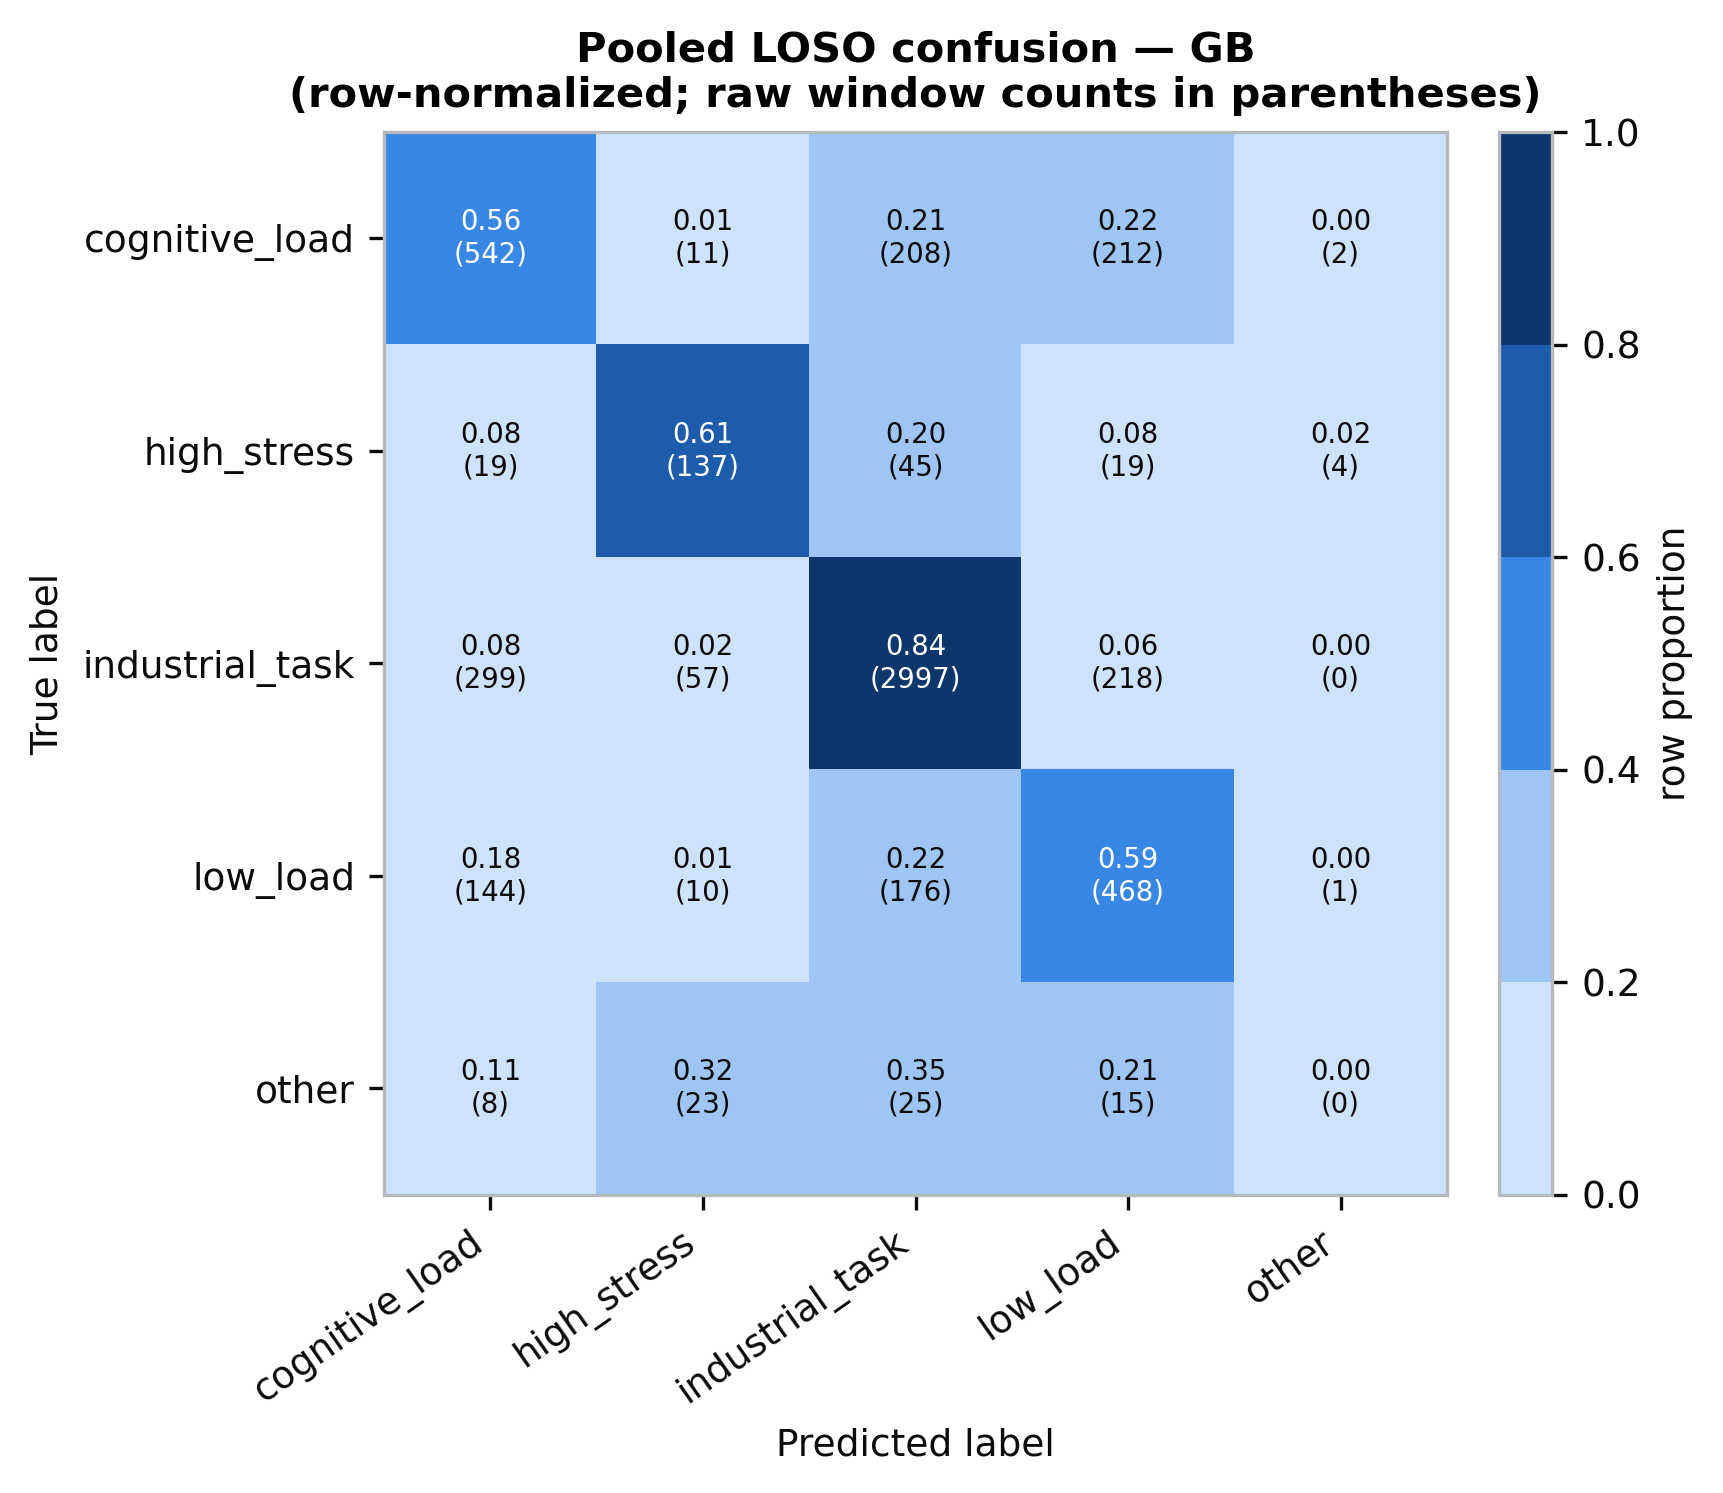
\includegraphics[width=0.72\textwidth]{fig1_confusion_loso.png}
\caption{Pooled \ac{OOF} confusion matrix of the best \ac{LOSO} model, row-normalized,
with raw window counts. Values are computed by summing the 52 per-operator fold
matrices before normalizing.}
\label{fig:confusion}
\end{figure}

\begin{figure}[t]
\centering
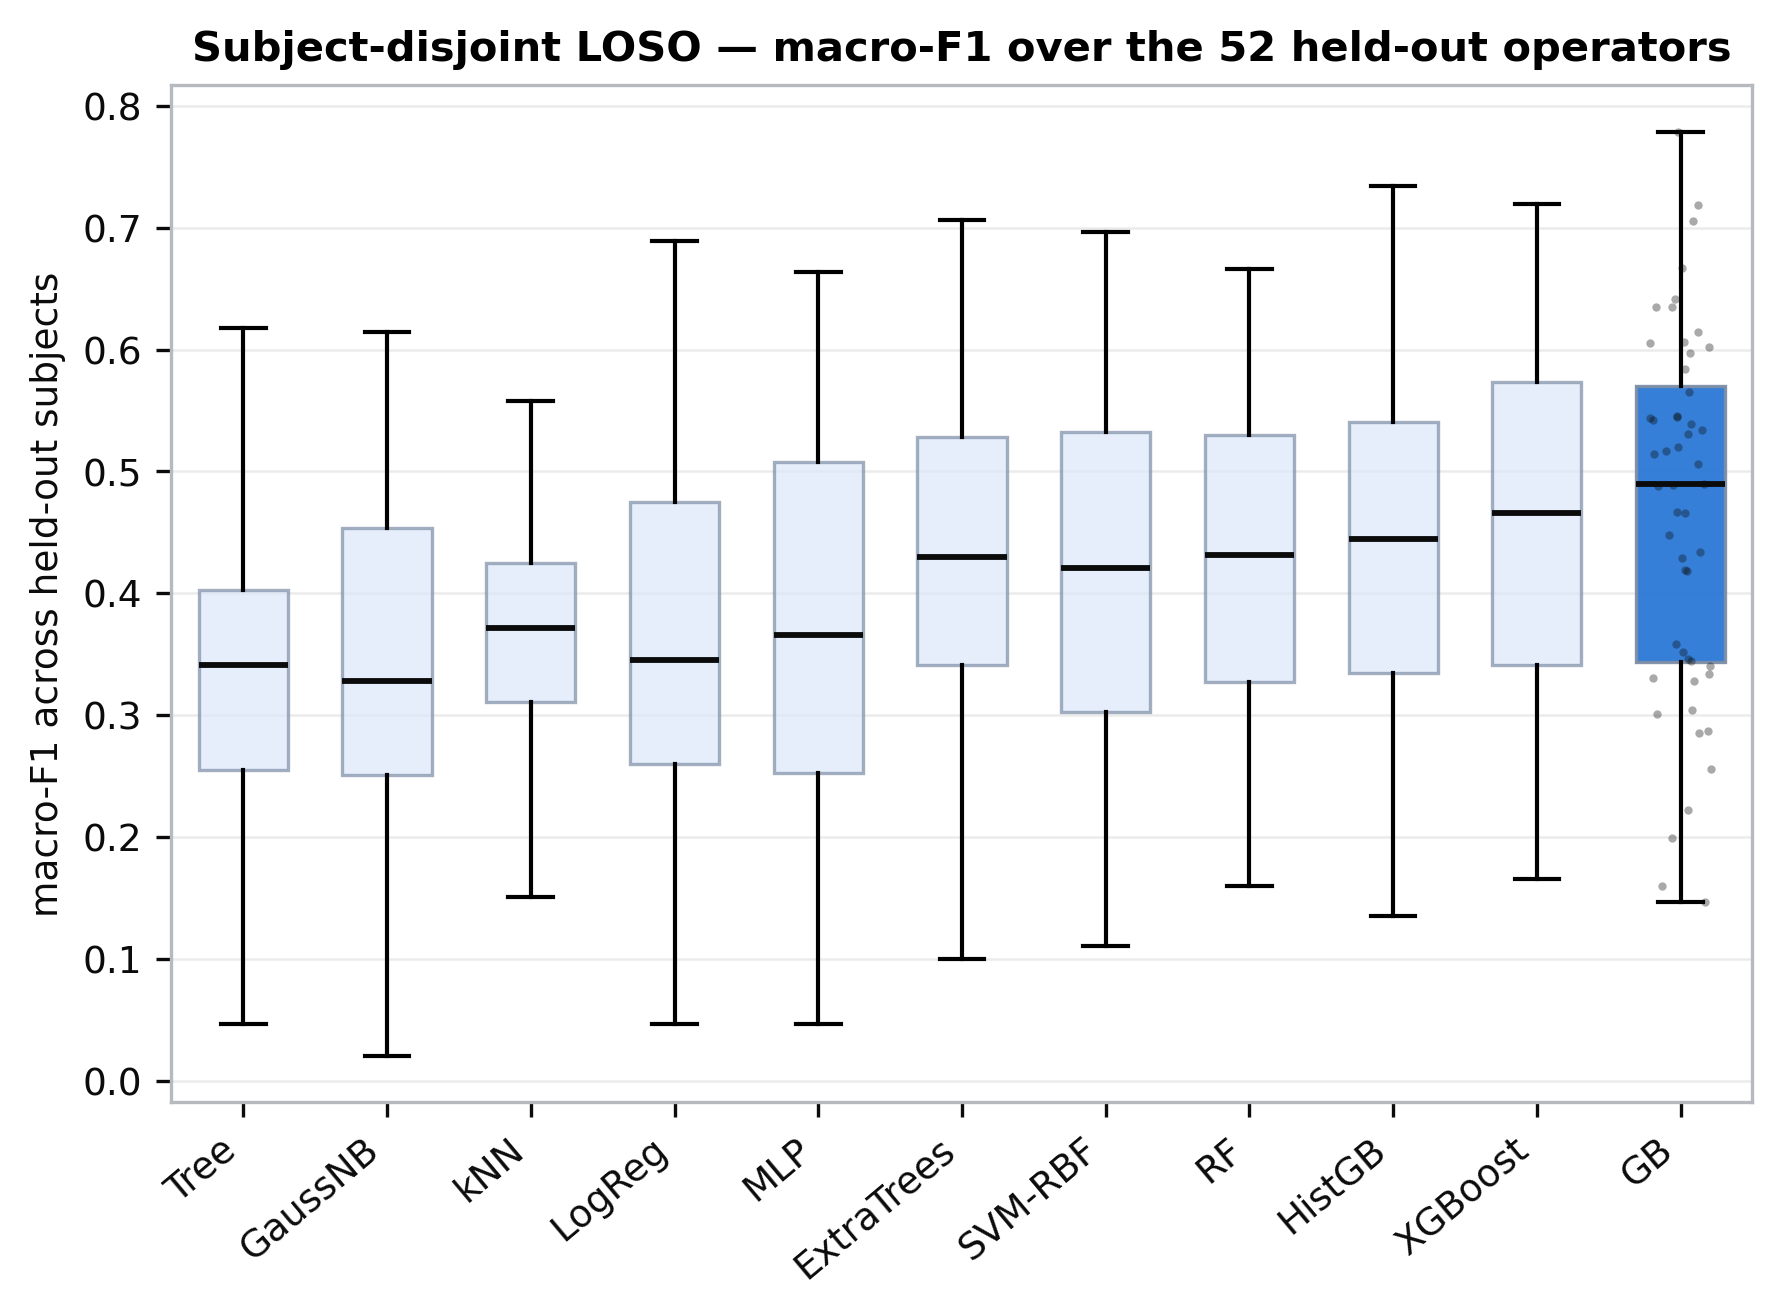
\includegraphics[width=\textwidth]{fig3_loso_subject_box.png}
\caption{Distribution of per-operator macro-F1 for every detector under \ac{LOSO}.
Each box summarizes the 52 held-out operators. Large spread means the detector's
usefulness depends strongly on which operator it meets.}
\label{fig:subject}
\end{figure}

Figure~\ref{fig:subject} reveals the second main finding: per-operator macro-F1 varies
widely, from 0.15, barely above the 0.2 chance floor for a five-class problem, to 0.78
across the 52 operators. A detector that works well for one operator can be
near-useless for another, and this variance, not the mean, is the practical obstacle
to assistive deployment. It is also the mechanism behind the generalization gap
quantified next, and it motivates the personalization discussion in
Section~\ref{sec:discussion}.

\subsection{The generalization gap}

Table~\ref{tab:gap} and Figure~\ref{fig:gap} contrast the within-subject ceiling with
the \ac{LOSO} result on the identical features. The within-subject classifiers reach
$0.91$ macro-F1, with \ac{XGBoost} at 0.910 and HistGB at 0.911, against
$0.45$--$0.46$ across
operators for the same models, a gap of roughly $0.45$ points.

\begin{table}[t]
\centering
\small
\caption{Generalization gap on the identical clean features. Within-subject is a
stratified random 80/20 split, in which the same operators appear in both training
and test, an optimistic ceiling, while LOSO holds whole operators out. The gap
quantifies how much performance is lost when no data from the target operator is
available at training time.}
\label{tab:gap}
\begin{tabular}{lccc}
\toprule
Model & Within-subject & LOSO & Gap \\
\midrule
XGBoost & 0.910 & 0.462 & +0.448 \\
HistGB & 0.911 & 0.451 & +0.459 \\
RF & 0.877 & 0.430 & +0.447 \\
MLP & 0.846 & 0.374 & +0.472 \\
\bottomrule
\end{tabular}
\end{table}


\begin{figure}[t]
\centering
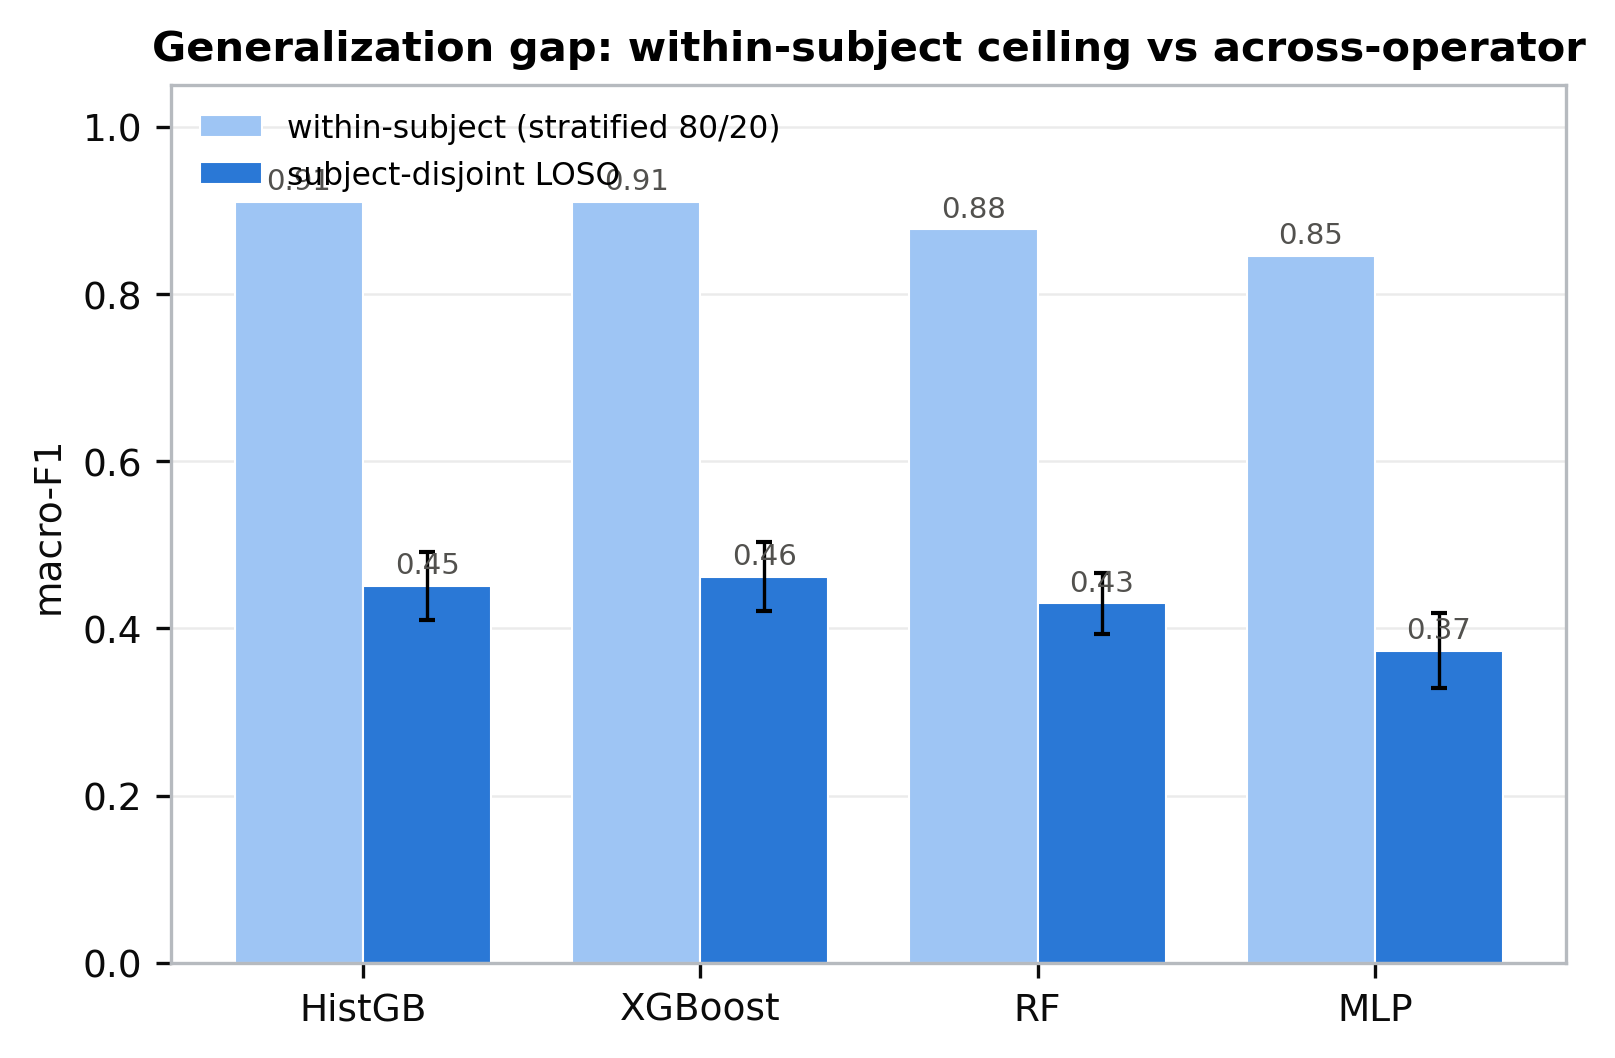
\includegraphics[width=0.72\textwidth]{fig5_generalization_gap.png}
\caption{Within-subject ceiling versus across-operator \ac{LOSO} macro-F1 on identical
features. The gap quantifies how much performance is lost when the target operator was
absent from training.}
\label{fig:gap}
\end{figure}

This gap is the headline finding of the paper and the reason row-level evaluations of
physiological windows are misleading: most of the apparent accuracy of a row-level
split reflects \emph{recognizing the person}, not the task state. The mechanism is the
per-operator physiological signature: baselines and response magnitudes that differ
sharply between individuals. An assistance system deployed on a new operator without
any calibration data should therefore expect performance near the lower, \ac{LOSO}
numbers, not the within-subject ones.

\subsection{Does fusion help?}

Table~\ref{tab:ablation} and Figure~\ref{fig:ablation} answer the modality question
under the same protocol: for each leading model we run \ac{EEG}-only, peripheral-only,
and fused inputs with 96, 32, and 128 features respectively. Peripheral physiology
alone already beats \ac{EEG} alone by a wide margin, for example \ac{XGBoost} reaches
$0.39$ versus $0.33$, yet adding \ac{EEG} on top of the periphery still helps: fused
improves over the best single modality for all four models, by $+0.072$ for
\ac{XGBoost} with $p<10^{-4}$, $+0.050$ for HistGB with $p = 0.002$, $+0.047$ for RF
with $p = 0.015$, and $+0.037$ for MLP with $p = 0.105$, which is not significant. The
two-tower network, which fuses through separate modality towers rather than
concatenation, reaches $0.406 \pm 0.158$, above fused \ac{MLP} and every
single-modality input but significantly below fused \ac{XGBoost}, by $-0.056$ with
$p = 0.001$.

\begin{table}[t]
\centering
\small
\caption{Benefit of feature fusion under the identical 52-subject LOSO protocol.
Fused 128-dimensional input is compared with the better single modality, EEG-only or
physio-only, per model. \emph{p}-values are paired Wilcoxon signed-rank tests over
the 52 folds. Two-Tower is the neural model with explicit per-modality towers,
compared with fused XGBoost.}
\label{tab:ablation}
\begin{tabular}{lccccc}
\toprule
Model & Best single & Single & Fused & $\Delta$ & Wilcoxon $p$ \\
\midrule
XGBoost & physio & 0.390 & 0.462 & +0.072 & 0.000 \\
HistGB & physio & 0.401 & 0.451 & +0.050 & 0.002 \\
RF & physio & 0.383 & 0.430 & +0.047 & 0.015 \\
MLP & physio & 0.337 & 0.374 & +0.037 & 0.105 \\
Two-Tower $vs$ fused XGB & fused XGB & 0.462 & 0.406 & -0.056 & 0.001 \\
\bottomrule
\end{tabular}
\end{table}


\begin{figure}[t]
\centering
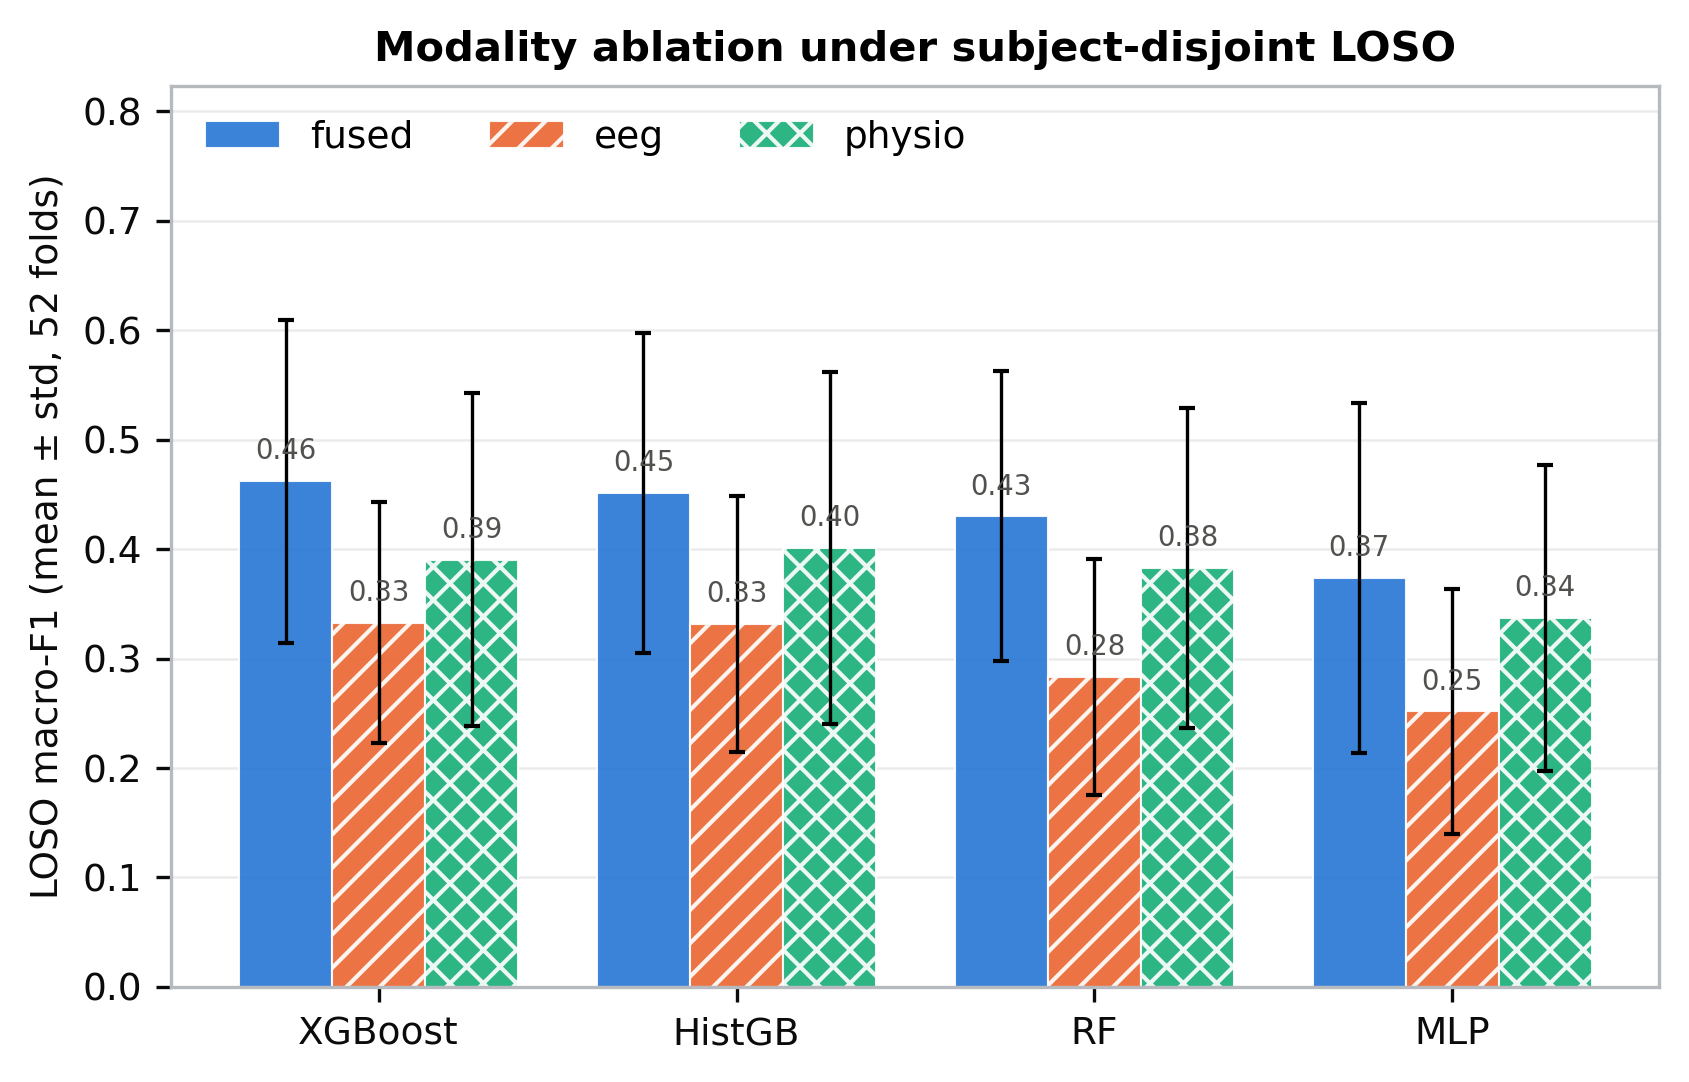
\includegraphics[width=0.8\textwidth]{fig4_modality_ablation.png}
\caption{Modality ablation under \ac{LOSO}: fused, \ac{EEG}-only, and peripheral-only
inputs with 128, 96, and 32 features respectively for the leading detectors. Error
bars are the standard deviation over the 52 folds.}
\label{fig:ablation}
\end{figure}

This result matters for the fusion literature. On this data, the gains from combining
central and peripheral physiology are real and statistically significant for the
leading models, but they are an order of magnitude smaller than the operator effect
that dominates the error budget. In other words, fusion helps, but it is not the
bottleneck: an explicit two-tower architecture adds nothing over plain
concatenation fed to a strong tree ensemble, a useful negative result for
practitioners choosing between simple and structured fusion.

\subsection{Statistical significance}

Figure~\ref{fig:significance} reports the per-fold paired Wilcoxon comparison of every
detector against the best, gradient boosting. Under the across-operator protocol, the
top three tree ensembles are statistically indistinguishable: \ac{XGBoost} at
$p = 0.88$, HistGB at $p = 0.38$, while random forest and extra trees separate only
at $p = 0.018$ and $p = 0.003$. By contrast, the gap between the tree ensembles and
the linear/instance-based/neural group is decisive: every member separates from the
best at $p \le 3\times10^{-5}$, and most below $10^{-6}$. Together with the effect
sizes, this tells the reader which reported differences are worth acting on.

\begin{figure}[t]
\centering
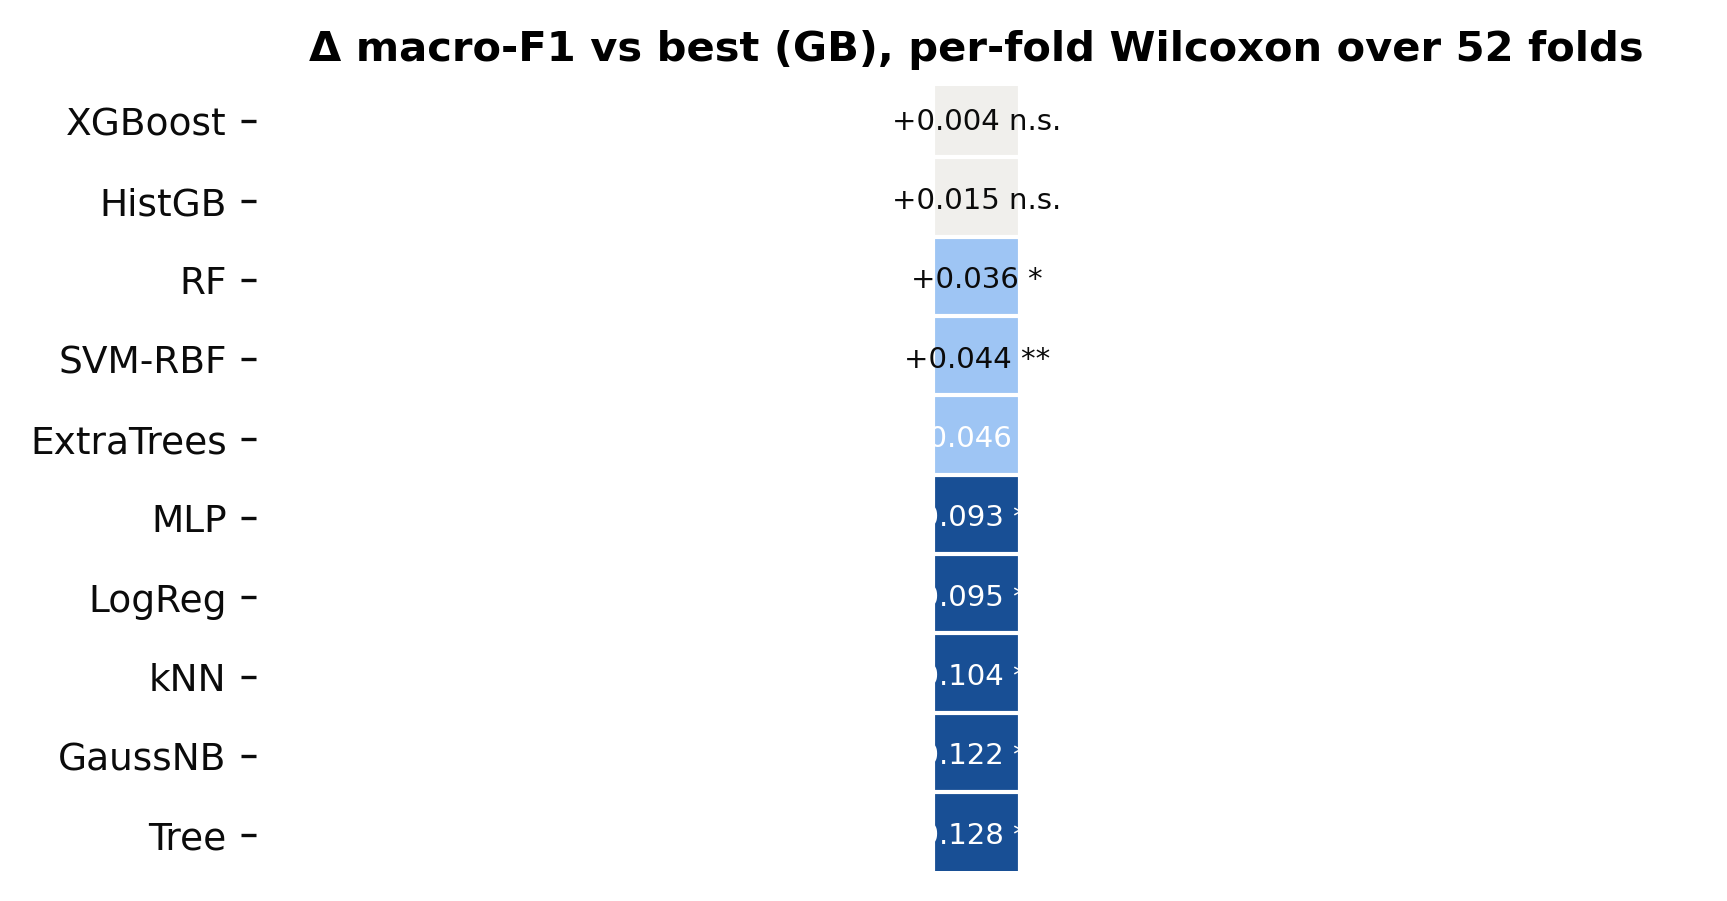
\includegraphics[width=0.75\textwidth]{fig6_significance.png}
\caption{Mean macro-F1 difference of each detector relative to the best, with the
paired Wilcoxon significance over the 52 folds.}
\label{fig:significance}
\end{figure}

\subsection{Real-time feasibility}

The sensor windows last on the order of tens of seconds, while all evaluated detectors
classify a single window in roughly 2--90\,$\mu$s of CPU time, about
5\,$\mu$s for the best detector and 19\,$\mu$s for \ac{XGBoost}, as listed in
Table~\ref{tab:benchmark}. Inference is therefore orders of magnitude faster than
real time on commodity CPUs, and real-time adaptive assistance is not constrained by
inference cost but by the reliability question of Section~\ref{sec:discussion}.

\section{Discussion}
\label{sec:discussion}

Taken together, our results reveal three important insights about recognizing operator
task states from physiological signals in \ac{HRC}.

\emph{First, the honest across-operator numbers are low, and the gap to the
within-subject ceiling is the real result.} The best detector reaches $0.466$ macro-F1
under \ac{LOSO}, while the same features with a row-level split report $0.91$, a gap
we reproduce with a stratified within-subject split and then explain as leakage of
operator identity. We consider the \ac{LOSO} figure the only defensible headline, and
we recommend that physiological-recognition papers report the within-subject ceiling
and the across-operator result \emph{together}, as in Table~\ref{tab:gap}. Reporting
either alone is misleading in opposite directions.

\emph{Second, three factors make the problem hard, and none is fixable by a better
classifier alone.} Firstly, \emph{the operator effect dominates}: physiological
baselines and gains differ so much between people that a model cannot separate ``this
operator is stressed'' from ``this operator responds strongly'' without calibration
data \cite{aygun2022assistive,borghi2025operatorstress}. Secondly, \emph{the classes
are coarse but confusable}: cognitive-load and industrial-task conditions plausibly
share attentional and motor components, so confusion between them is physiologically
reasonable. Thirdly, \emph{the imbalance is extreme at the tail}: two minority
classes have 224 and 71 windows spread over very few conditions, making them
statistically near-impossible to learn across operators.

\emph{Third, fusion and speed are not the bottlenecks.} Fusing \ac{EEG} with
peripheral signals adds a real but small gain, namely $+0.072$ macro-F1 for the best
model, explicit two-tower fusion does not beat concatenation, and inference takes
microseconds per window. An assistive system is therefore not limited by what it can
compute or how it fuses, but by whether it has met the operator before. This reframing
points the research effort where it belongs: at personalization and at calibration of
the confidence that would gate assistance.

\subsection{Comparison with the source protocol}

Bussolan et al.\ report subject-disjoint recognition of \emph{self-reported} stress
and cognitive-load levels with macro-F1 around 0.34--0.49
\cite{bussolan2025multiphysiohrc,bussolan2024stressdetector}. Our numbers are not
directly comparable for two reasons: their targets come from STAI-Y1 / NASA-TLX
self-reports on a subset of conditions, whereas ours are deterministic
task-condition labels on all conditions, and their protocol concerns a narrower
assembly setting. Obtaining the dataset's questionnaire tables, which are not in the
public feature export we used, would let us map our task-condition predictions onto
the self-report levels and compare head-to-head. We flag this as the single most
valuable extension rather than claim comparability we cannot substantiate.

\subsection{Threats to validity}

\begin{itemize}
\item \textbf{Construct validity of labels.} Our labels are task conditions, not
measured mental states. A cognitive-load condition may not produce cognitive load in
every operator at every window: the label is a \emph{protocol} label. We state this
explicitly and never equate a prediction with a diagnosis.
\item \textbf{Class-size and condition confound.} The \emph{other} class is a single
condition, 71 windows, so a detector can effectively memorize that condition. Its
recall is reported only for transparency.
\item \textbf{Within-condition autocorrelation.} Even under \ac{LOSO}, a test fold
contains consecutive windows of the same condition from one operator. Per-fold scores
are per-operator estimates, not independent samples. Our paired tests respect this by
pairing per-operator scores. The pooling step of Section~\ref{sec:protocol} is
descriptive, not an independence claim.
\item \textbf{Feature provenance.} We cleaned the exported feature table we obtained.
We did not recompute features from raw signals. The manifest makes the cleaning
reproducible, but the upstream feature computation is the dataset authors'.
\item \textbf{Sensor placement and recording hardware} are fixed by the dataset and
were not varied, so results may not transfer to different hardware or real factory noise,
where motion artefacts would be larger than in a laboratory \ac{HRC} setting.
\end{itemize}

\subsection{Deployment considerations}

Physiological sensing in the workplace raises privacy and acceptability questions that
are not technicalities. \ac{EEG} headsets and physiological wearables capture
information far beyond task state, and continuous monitoring of stress in industrial
settings can be used for worker surveillance rather than assistance. Any deployment
should, first, process signals on-device where feasible and retain only task-state
decisions, second, use predictions to \emph{adapt robot behaviour}, never for
individual performance evaluation, and third, make the operator's right to opt out and
to know what is inferred explicit. A failure/fallback policy is equally important:
because confidence is currently unevenly calibrated, as shown in
Section~\ref{sec:results}, assistance
must degrade gracefully, falling back to a fixed, safe robot policy whenever the
detector's confidence is low, rather than acting on a low-confidence state estimate.

\section{Conclusion and Future Work}
\label{sec:conclusion}

Using physiological signals to drive adaptive assistance in industrial \ac{HRC}
requires recognizing what the operator is doing across people, not just within the
people a model was trained on. The central difficulty is that physiological baselines
and response magnitudes differ sharply between individuals, so an evaluation that does
not separate operators reports a ceiling rather than a generalization result, and the
between-operator variability that dominates real deployments goes unquantified.

To solve this problem, this paper proposes a leakage-free, strictly subject-disjoint
benchmark of task-state recognition on the public MultiPhysio-\ac{HRC} dataset. The
study rests on three components: first, a cleaning protocol that removes recording
metadata and duplicated \ac{EEG} exports, leaving 128 physiological features labelled
deterministically into five task-condition classes, second, an evaluation of eleven
detectors and one neural fusion network under a \ac{LOSO} protocol over all 52
operators, with every preprocessing step refit inside each fold, and third, a
modality-contribution analysis that tests, under the identical protocol, whether
fusing central and peripheral physiology helps.

Our evaluation shows the honest and reproducible picture. The best detector, gradient
boosting, reaches a per-fold macro-F1 of $0.466 \pm 0.149$ across new operators, and
within-subject classifiers on the identical features reach $0.91$, a generalization
gap of roughly $0.45$ points that dwarfs the differences between models. Fusion adds a
real but small gain, namely $+0.072$ for the best model, explicit fusion architecture
adds nothing over concatenation, and inference takes microseconds per window. These are the
properties an assistance system actually faces when it meets an operator for the first
time, and they explain why optimistic row-level evaluations of physiological windows
do not transfer to new operators.

Future work will pursue three directions. First, \emph{Personalization}: given the
operator effect, few-shot calibration, a handful of labelled windows from a new
operator, either as adaptation data or as a per-operator prior, is the most direct
route to usable accuracy, and our per-operator score files make the potential gain
measurable. Second, \emph{Self-report targets}: obtaining the dataset's questionnaire
tables would let us bridge the task-condition schema to the STAI/NASA-TLX stress and
cognitive-load levels used by the source authors, enabling the direct comparison we
currently flag as out of scope. Third, \emph{Temporal context}: the present work
classifies windows independently. Modelling the condition sequence and per-operator
dynamics with recurrent or state-space models is a natural next step, and the latency
headroom we measure leaves ample room for such models at inference time.

\bibliographystyle{splncs04}
\bibliography{task_type_detection_references}

\end{document}
